\section{Introduction}

\begin{frame}
	\frametitle{Introduction}
	\vspace{-10ex}
	The root-locus method dealt with the s- and z-domains and the location of the poles and zeros formed the basis for that method.\\
	\medskip
	For the \textbf{frequency domain}, we use the following substitution: $s=j\omega$, which means we will only regard perfect oscillations.\\
	\medskip
	Sines, cosines and exponential signals are eigenfunctions of Linear Time Invariant systems (LTI).\\
	Perfect oscillations form the natural decomposition of each signal when you are dealing with LTIs.
\end{frame}

\begin{frame}
	\frametitle{Introduction}
	We need to translate our \textbf{design criteria} to something that fits the discussed method. For the root-locus method, we had to express the criteria in positions of poles and zeros.\\
	For the frequency domain, typical design criteria are:
	\begin{itemize}
		\item Phase and gain margin
		\item Bandwidth
		\item Zero-frequency magnitude (= DC gain)
	\end{itemize}
	\bigskip
	We will discuss two different \textbf{graphical representations} to design compensators in the frequency domain:
	\begin{itemize}
		\item Nyquist plots
		\item Bode plots (for the design of lead, lag and lead-lag compensators: next lecture)
	\end{itemize}
\end{frame}

\section{Stability}

\begin{frame}
	\frametitle{Stability of the closed loop system}
	\begin{figure}
		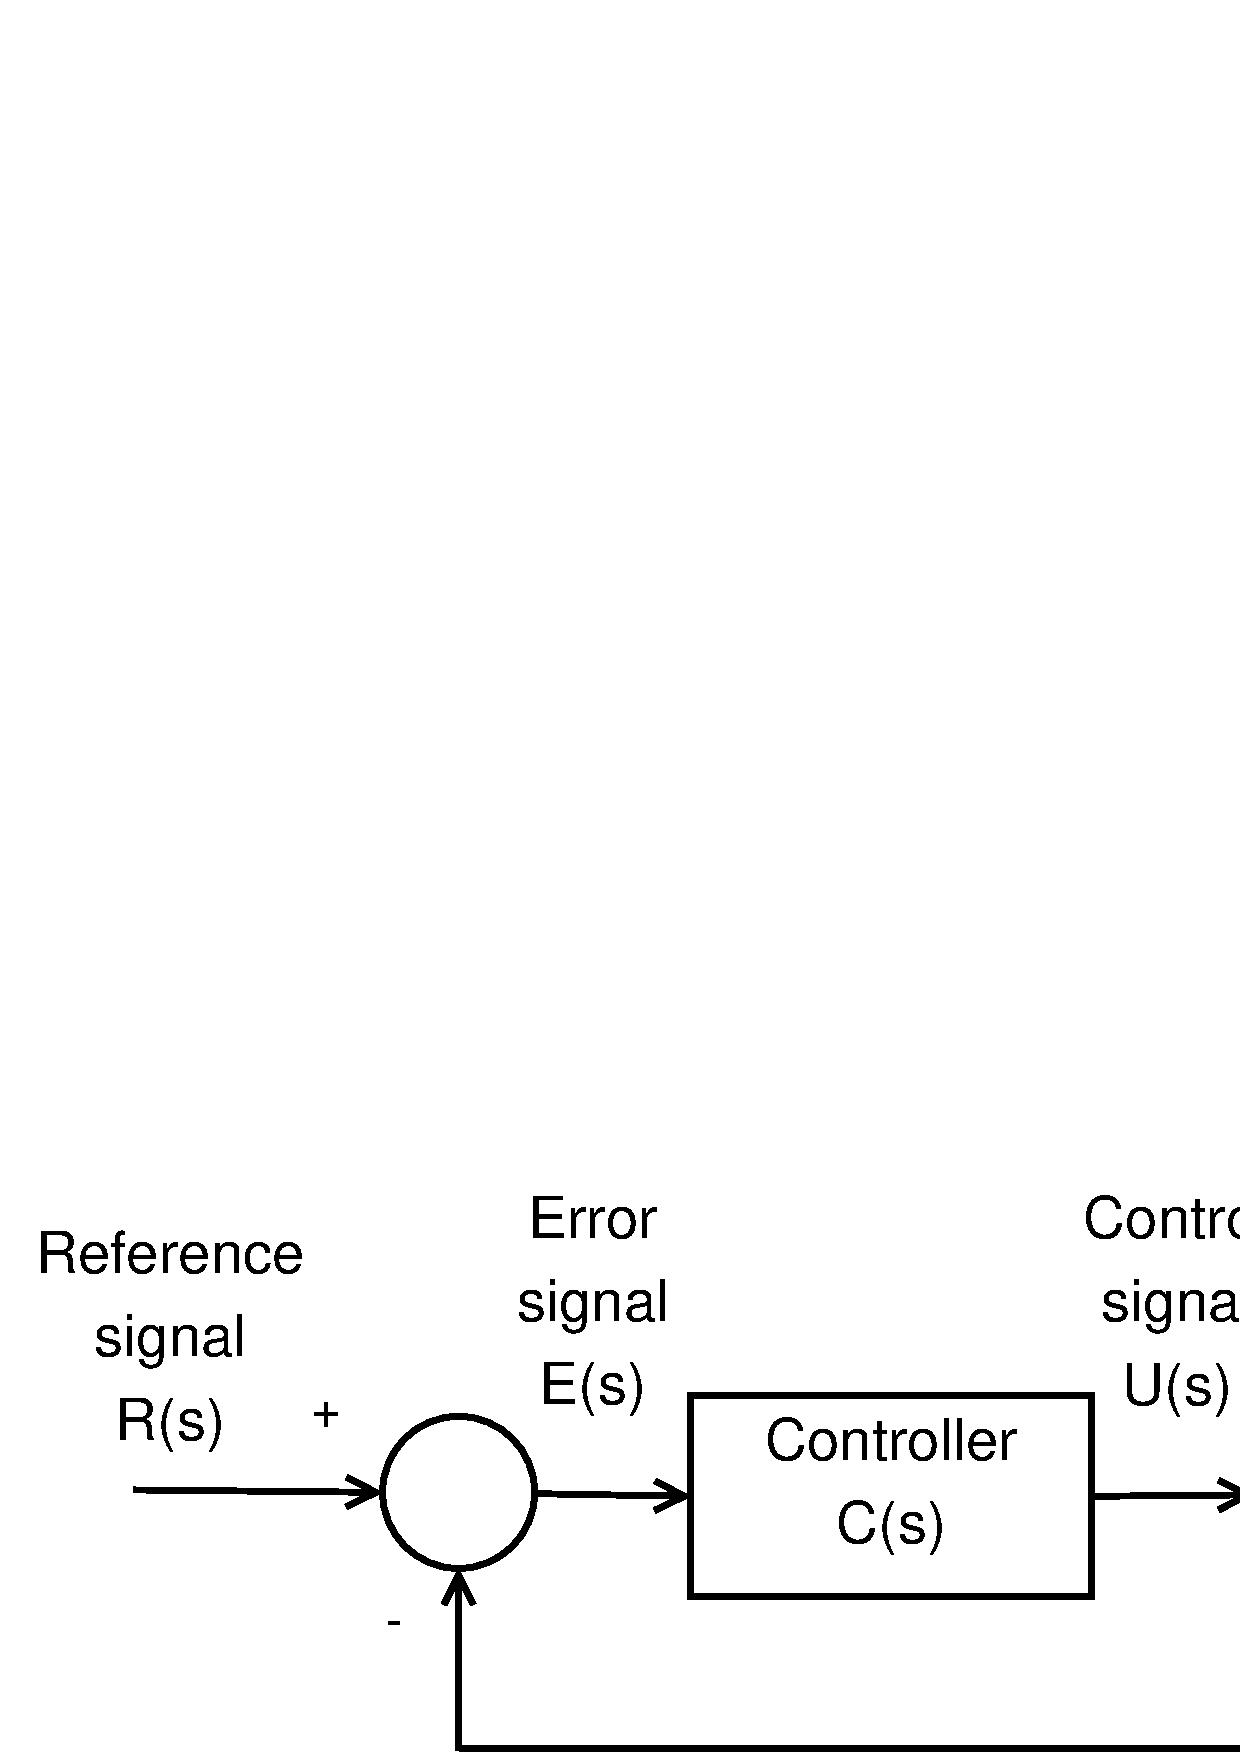
\includegraphics[width=0.8\linewidth]{closedloop}
	\end{figure}
	We write the output signal as a function of the input signal: $$Y(s)=\frac{P(s)C(s)}{1+P(s)C(s)}R(s).$$\\
	The closed loop system stability is determined by the poles of $\frac{P(s)C(s)}{1+P(s)C(s)}$, or the roots of $1+P(s)C(s)=0$.
\end{frame}

\begin{frame}
	\frametitle{Stability of the closed loop system}
	\vspace{-8ex}
	In the root-locus method, we determined the positions of the poles by plotting the roots of $1+P(s)C(s)=0$.\\
	\medskip
	The system is stable if all the roots remain in the left half plane.\\
	\medskip
	We are however not interested in the positions of the poles.\\
	We only need to know whether there \textit{are} poles in the right half plane.\\
	\medskip
	There is a cheaper alternative: \textbf{the Nyquist stability criterion}.
\end{frame}

\begin{frame}
	\frametitle{Stability: Nyquist criterion}
	\vspace{-5ex}
	The Nyquist stability criterion avoids determining the roots of $1+P(s)C(s)$ exactly. It only determines the \textit{number} of roots in the right half plane.\\
	\medskip
	It uses a theorem from complex calculus that finds the difference between the number of poles and the number of zeros within a \textbf{contour} (a closed curve).\\
	\medskip
	We will apply this theorem to $1+P(s)C(s)$ (which can be seen as a complex function) and the contour will encircle the entire right half plane (= \textbf{the Nyquist contour}).
\end{frame}

\section{Cauchy's argument principle}

\subsection{Cauchy's argument principle}

\begin{frame}
	\frametitle{Complex function}
	Before we get to the theorem, we discuss the concept of a complex function.\\
	\smallskip
	A complex function $f(s)=u(x,y)+\mathit{j}v(x,y)$ maps the complex number $s=x+\mathit{j}y$ onto the complex number $w=u+\mathit{j}v$.
	\vspace{-2ex}
	\begin{columns}
		\column{0.5\textwidth}
		\begin{center}
			For a complex number:
		\end{center}
		\begin{figure}
			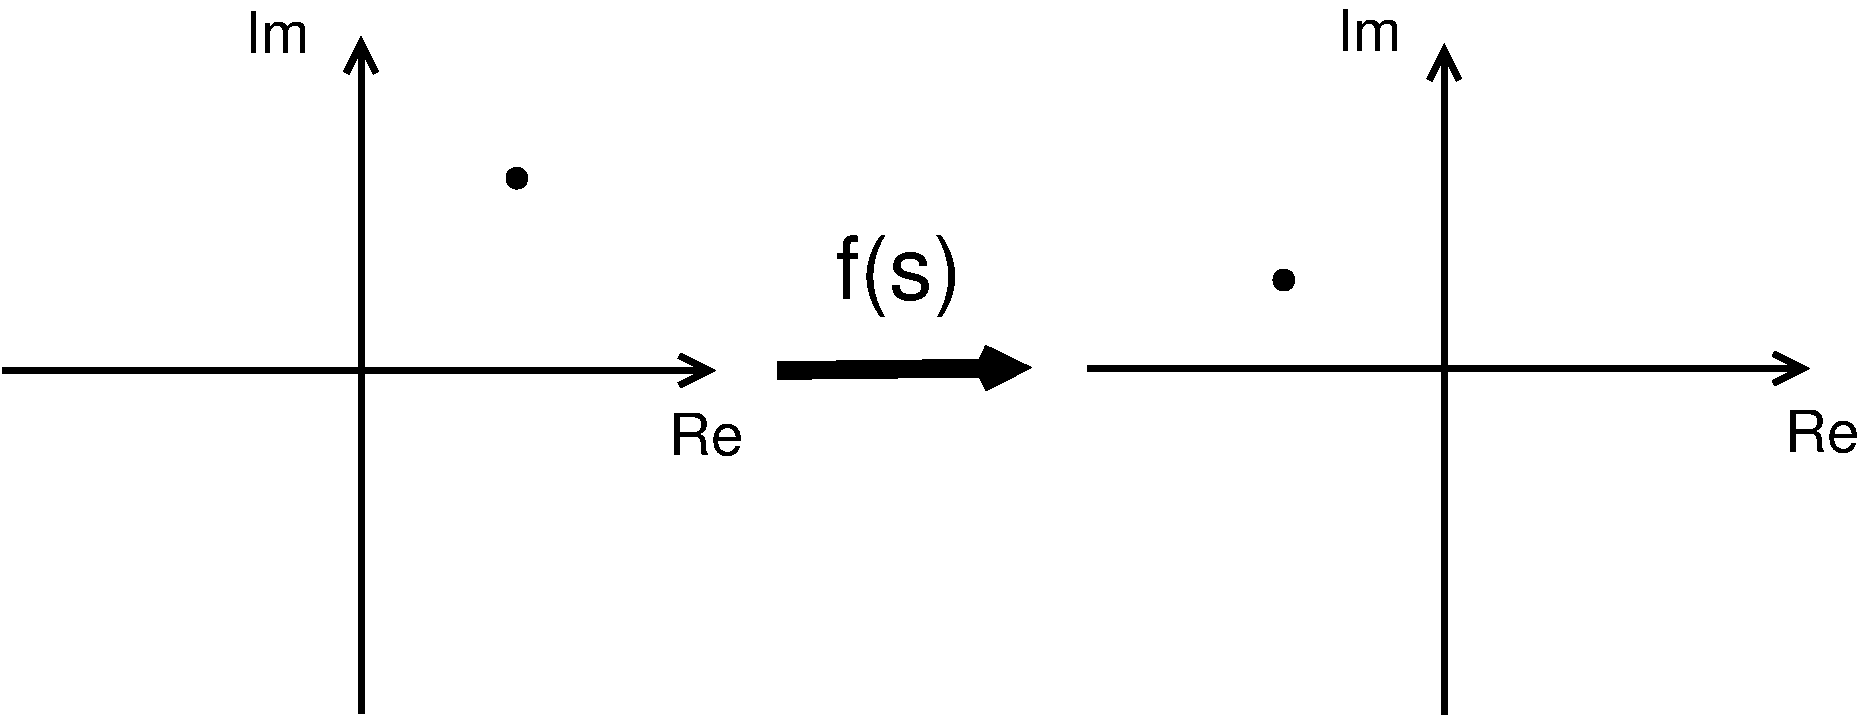
\includegraphics[width=1.0\linewidth]{complex1}
		\end{figure}
		\column{0.5\textwidth}
		\begin{center}
			or for a contour:
		\end{center}
		\begin{figure}
			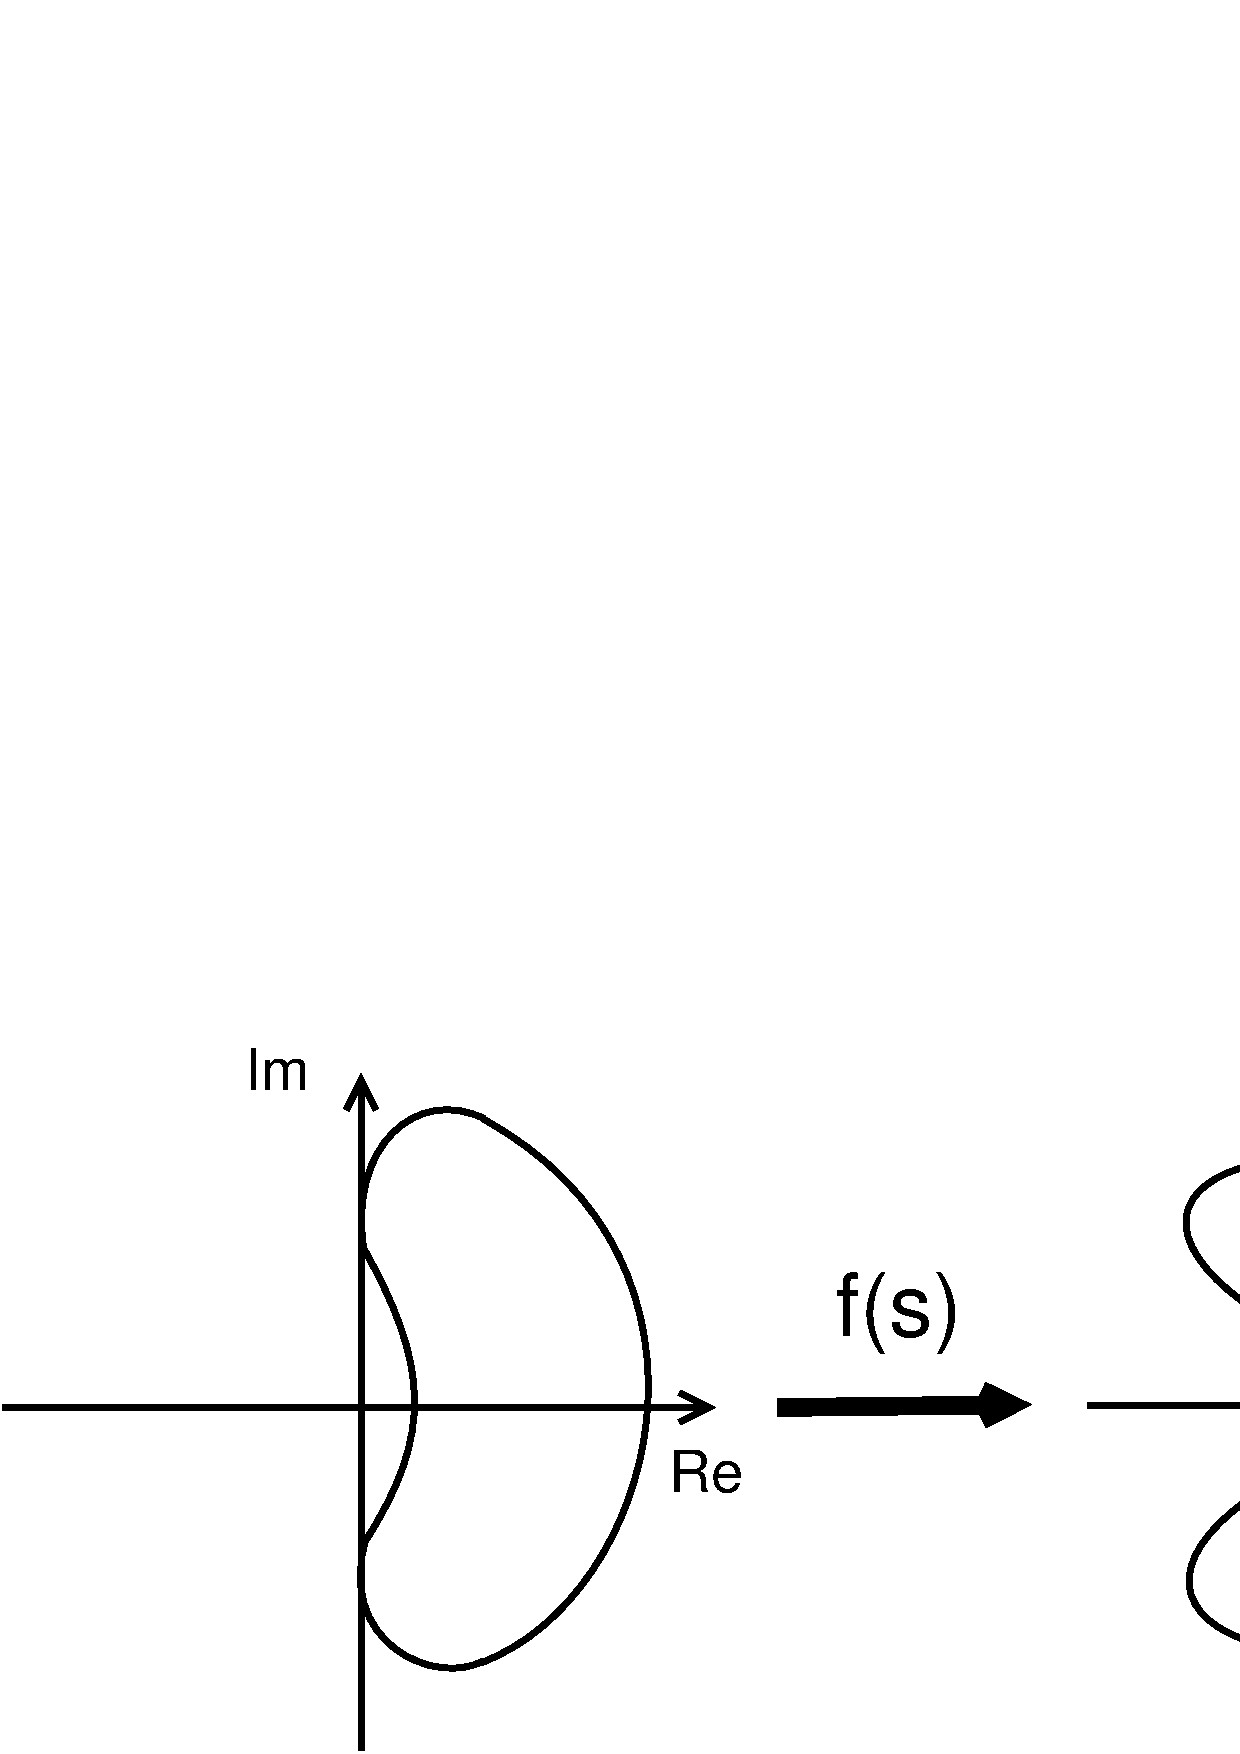
\includegraphics[width=1.0\linewidth]{complex2}
		\end{figure}
	\end{columns}
	\medskip
	The function $1+P(s)C(s)$ can also be regarded as a complex function, so we can use it as a mapping.
\end{frame}

\begin{frame}
	\frametitle{Cauchy's argument principle}
	\vspace{-7ex}
	This is the engine behind the Nyquist stability criterion.\\
	\medskip
	If a contour $\Gamma$ in the s-plane encircles Z zeros and P poles of $f(s)$ in clockwise direction, the contour $\Gamma'$, which is the image of $\Gamma$ as mapped by $f(s)$, encircles the origin (in the w-plane) $Z-P$ times in the clockwise direction.\\
	\medskip
	So the only thing we are looking at is the \textbf{number of encirclements} of the origin. \\
	On the next slides, we will prove this.
\end{frame}

\begin{frame}
	\frametitle{Cauchy's argument principle}
	\vspace{-3ex}
	Let's take a complex function $f(s)=\frac{(s-z_1)(s-z_2)(s-z_3)...}{(s-p_1)(s-p_2)(s-p_3)...}$.\\
	\medskip
	If we would apply this function to a complex number c, this comes down to multiplying factors $c-z_i = A_{z_{i}}e^{j\theta_{z_{i}}}$ and $\frac{1}{c-p_i}=\frac{1}{A_{p_{i}}}e^{-j\theta_{p_{i}}}$.\\
	\medskip
	So the \textbf{modulus} of $f(c)$ can be easily found by evaluating $\frac{A_{z_{1}}A_{z_{2}}A_{z_{3}}...}{A_{p_{1}}A_{p_{2}}A_{p_{3}}...}$.	This might help if you want to map a point, but it is not important for us.\\
	\medskip
	The evaluation of the \textbf{argument} of $f(c)$ is what will be interesting: $\angle f(c) = \theta_{z_{1}}+\theta_{z_{2}}+\theta_{z_{3}}+...-\theta_{p_{1}}-\theta_{p_{2}}-\theta_{p_{3}}-...$
\end{frame}

\begin{frame}
	\frametitle{Cauchy's argument principle: graphically}
	\begin{figure}
		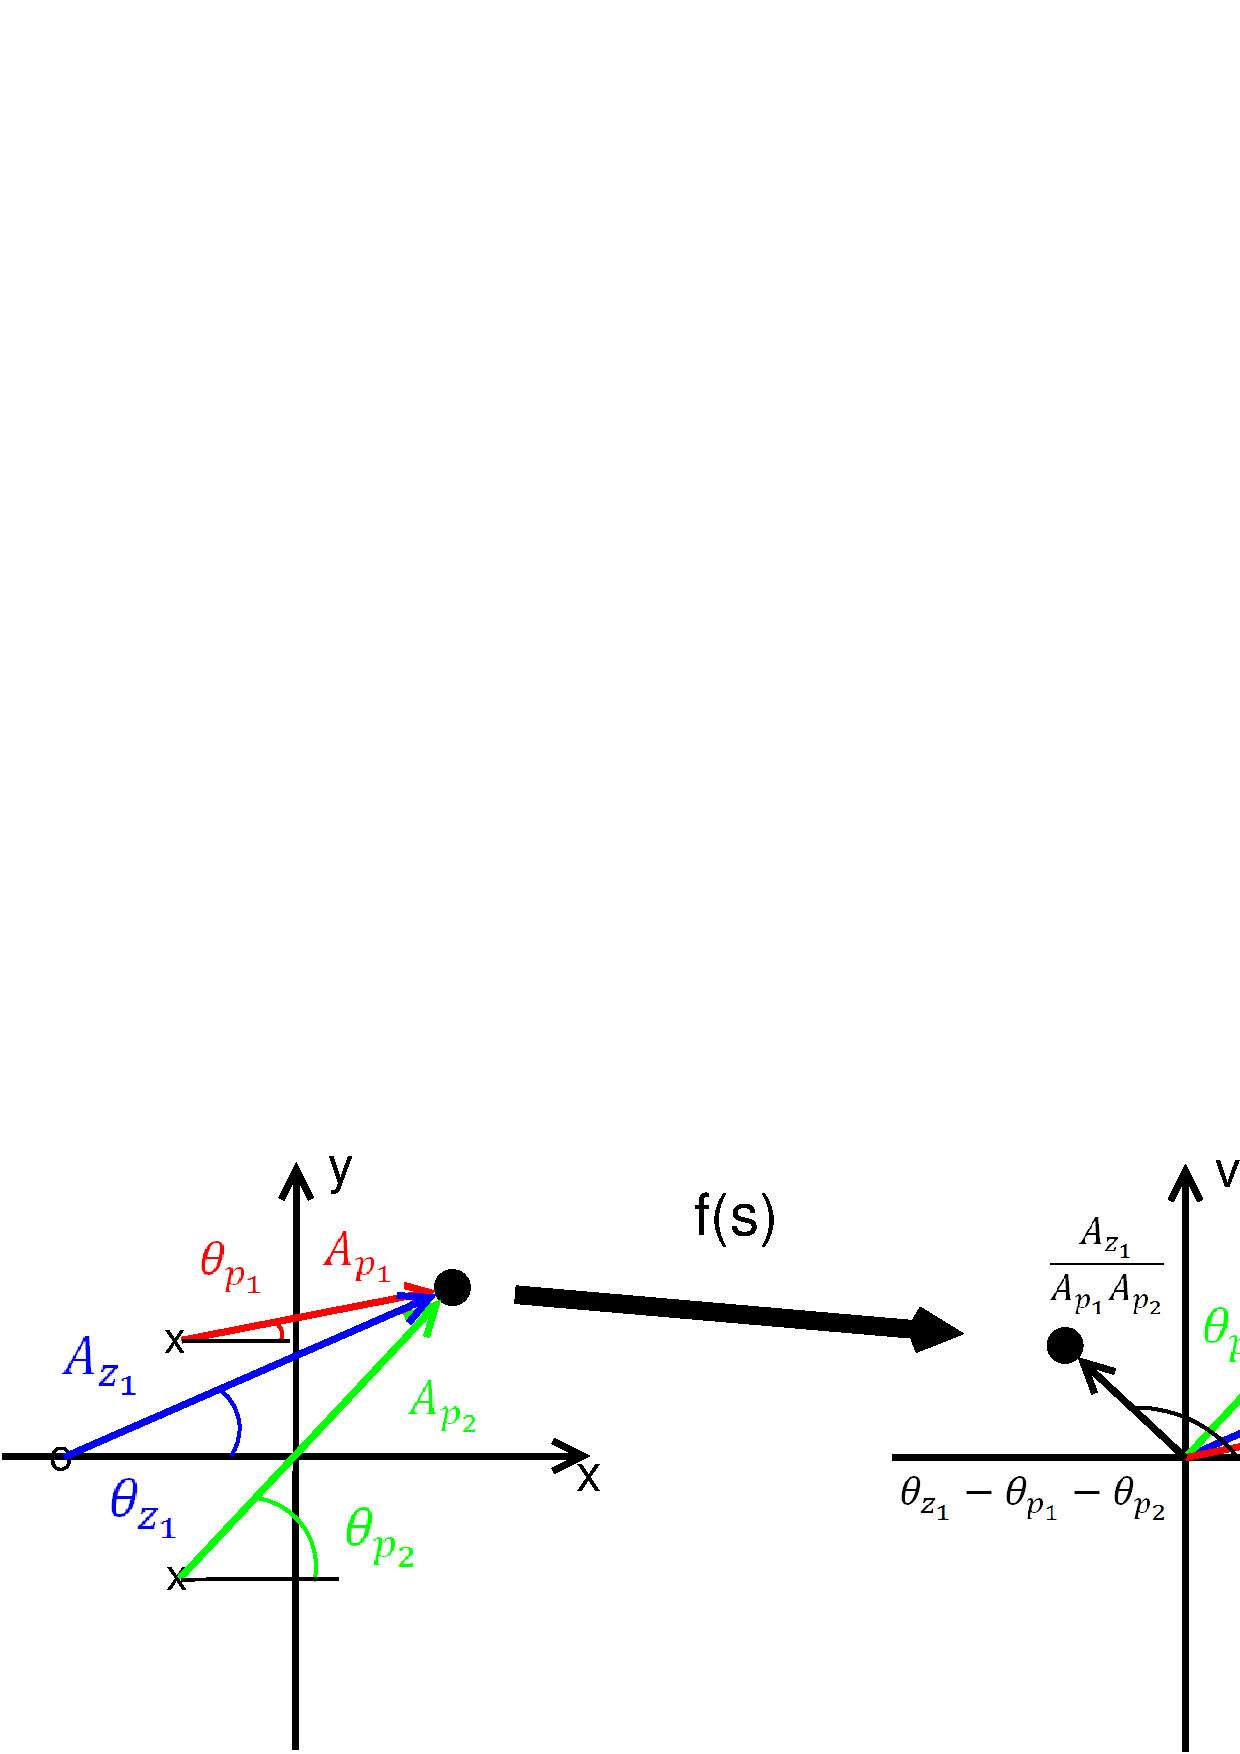
\includegraphics[width=1.0\linewidth]{graphical}
	\end{figure}
\end{frame}

\begin{frame}
	\frametitle{Cauchy's argument principle}
	When does the image of a contour in the w-plane encircle the origin?\\
	\medskip
	That happens when the argument of the image of the contour at the beginning and the end differ by $2\pi$.\\
	\medskip
	A pole or zero outside the contour will never have that effect. One inside the contour has the following effect:\\
	\medskip
	\begin{figure}
		
\includegraphics[width=1\linewidth]{argument}
	\end{figure}
\end{frame}

\begin{frame}
	\frametitle{Cauchy's argument principle}
	\vspace{-4ex}
	A pole results in $-2\pi$ (counterclockwise rotation), if the contour is followed clockwise.\\
	\medskip
	A zero results in $+2\pi$ (clockwise rotation).\\
	\medskip
	This follows from the sign of their effect: $\angle f(c) = \theta_{z_{1}}+\theta_{z_{2}}+\theta_{z_{3}}+...-\theta_{p_{1}}-\theta_{p_{2}}-\theta_{p_{3}}-...$\\
	\bigskip
	It is also possible that the origin is encircled when there are no poles or zeros in the contour (in the s-plane). But then the amount of clockwise encirclements equals the amount of counterclockwise encirclements, hence no net encirclements.
\end{frame}

\subsection{Examples}

\begin{frame}
	\frametitle{Example 1}
	\begin{itemize}
		\item Two encircled poles (the x's): $P=2$
		\item Four encircled zeros (the o's): $Z=4$
		\item Hence: $N = Z-P = 2$
		\item Indeed, the image of the contour encircles the origin twice in the w-plane (in clockwise direction).
	\end{itemize}
	\vspace{-2ex}
	\begin{figure}
		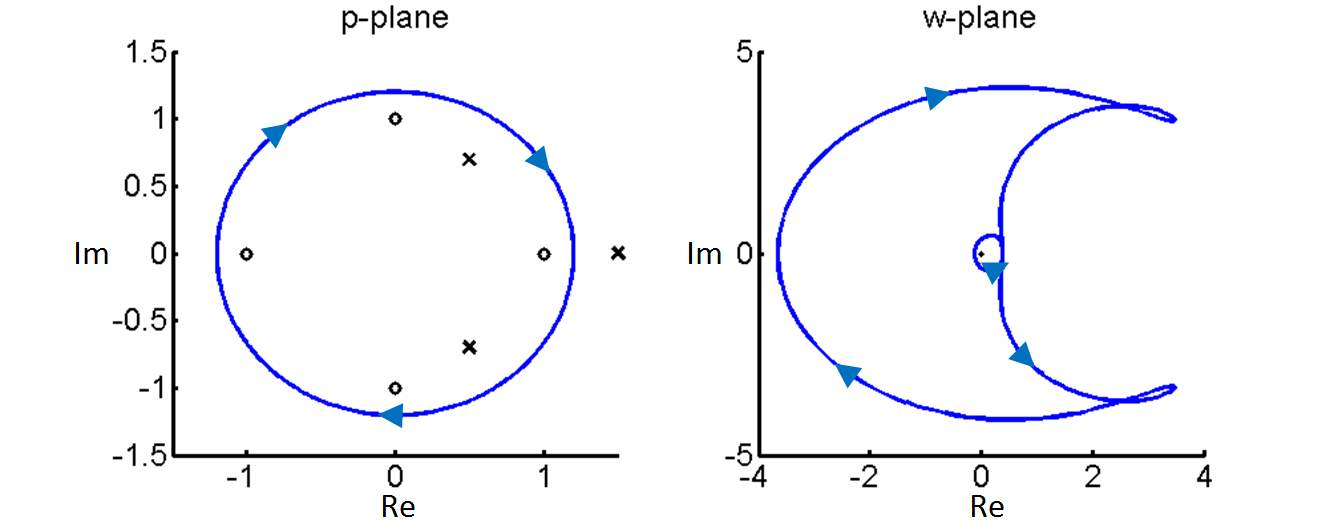
\includegraphics[width=0.95\linewidth]{example1}
	\end{figure}
\end{frame}

\begin{frame}
	\frametitle{Example 2}
	\begin{itemize}
		\item Two encircled poles: $P = 2$
		\item One encircled zero: $Z=1$
		\item Hence: $N=Z-P=-1$
		\item Indeed, the image of the contour encircles the origin once in the w-plane (in counterclockwise direction).
	\end{itemize}
	\vspace{-2ex}
	\begin{figure}
		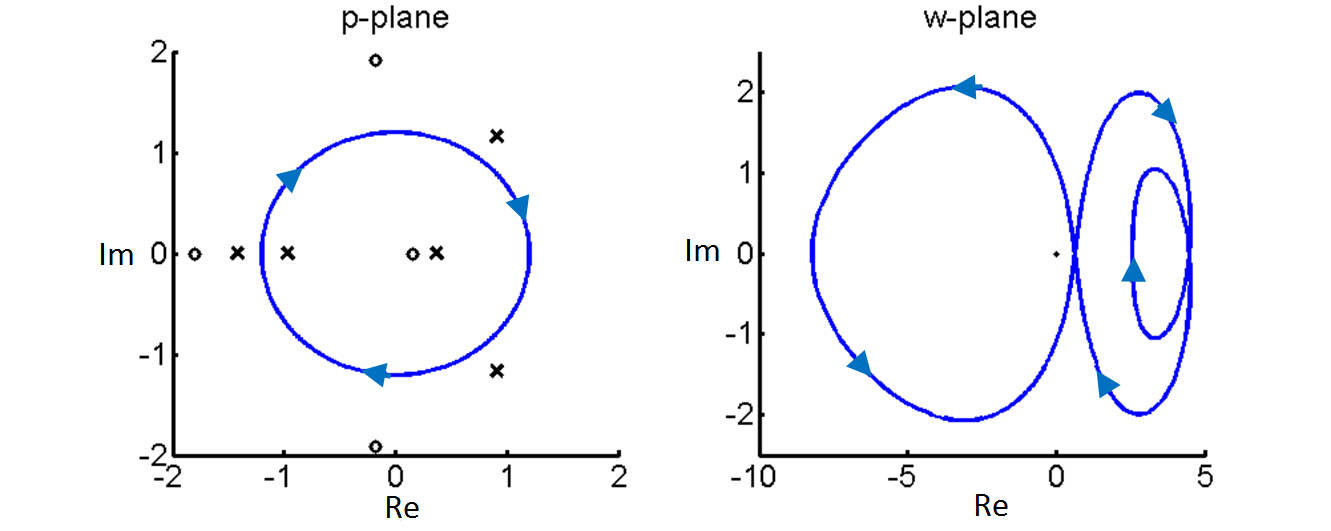
\includegraphics[width=0.95\linewidth]{example2}
	\end{figure}
\end{frame}

\section{Nyquist stability criterion}

\begin{frame}
	\frametitle{Nyquist stability criterion}
	If we apply Cauchy's argument principle to the following contour (the \textbf{Nyquist contour}), the amount of clockwise encirclements around the origin of the mapping of this contour (the \textbf{Nyquist plot}) in the w-plane equals $Z-P$ of the right half plane (RHP).
	\vspace{-1ex}
	\begin{figure}
		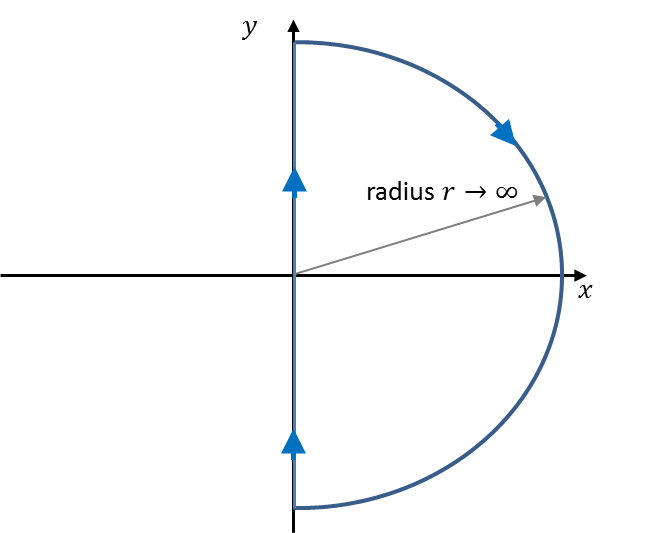
\includegraphics[width=0.35\linewidth]{nyquist_plot}
	\end{figure}
\end{frame}

\begin{frame}
	\frametitle{Nyquist stability criterion}
	That way, we will find the difference between the number of poles and zeros of $1+P(s)C(s)$ in the RHP: $N=Z-P$.\\
	\medskip
	So if we know P (the number of poles in the RHP of $1+P(s)C(s)$), we know how many roots of $1+P(s)C(s)$ there are in the RHP.
	\begin{figure}
		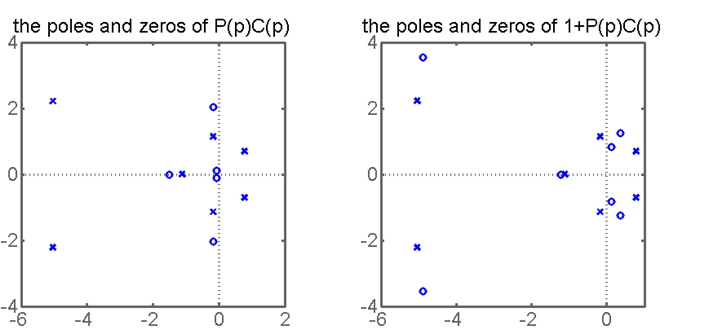
\includegraphics[width=0.8\linewidth]{pz}
	\end{figure}
\end{frame}

\begin{frame}
	\frametitle{Nyquist stability criterion}
	\vspace{-10ex}
	Luckily this last aspect is simple, since the roots of $1+P(s)C(s)$ equal those of $P(s)C(s)$. Hence the amount of RHP poles is equal (the connection between the zeros is not as clear).\\
	\bigskip
	So if the number of RHP poles of $P(s)C(s)$ is known (which is assumed), we know whether the system with unity (negative) feedback is stable.
\end{frame}

\begin{frame}
	\frametitle{Nyquist stability criterion}
	If we apply this to $1+P(s)C(s)$, we need to count the number of encirclements of the origin.\\
	However, the Nyquist stability criterion uses $P(s)C(s)$.
	\begin{itemize}
		\item The zeros of $1+P(s)C(s)$ and the poles and zeros of $P(s)C(s)$ are hard to relate.
		\item This is in sharp contrast with how easily the Nyquist plots relate: the Nyquist plot of $P(s)C(s)$ equals the one of $(1+P(s)C(s)$, after it has been moved to the right over a distance 1.
		\item To find $Z-P$, one has to count the number of clockwise encirclements of the image of $P(s)C(s)$ around the point $(-1,0)$, since this equals the number of clockwise encirclements of the image of $1+P(s)C(s)$ around the origin.
	\end{itemize}
\end{frame}

\begin{frame}
	\frametitle{Nyquist stability criterion}
	\begin{block}{Nyquist stability criterion}
		If the open loop system $P(s)C(s)$ has $\ell$ poles in the right half plane (of the s-plane), then the system with unity feedback is stable if and only if the Nyquist plot encircles the point (-1,0) $\ell$ times in the counter clockwise direction.
	\end{block}
\end{frame}

\section{Nyquist plot}

\subsection{Nyquist plot}

\begin{frame}
	\frametitle{Nyquist plot}
	We know how to deduce stability of the closed loop system from the Nyquist plot.\\
	Now we will discuss how these plots can be found.\\
	\smallskip
	First some simplifications:
	\vspace{-1ex}
	\begin{columns}
		\column{0.5\textwidth}
		\begin{enumerate}
			\item For physically realizable systems (i.e. relevant systems to engineers) the circle bow will be mapped on a point.
			\item The image of the positive imaginary axis is the mirror image of the negative imaginary axis
		\end{enumerate}
		\column{0.5\textwidth}
		\vspace{-2ex}
		\begin{figure}
			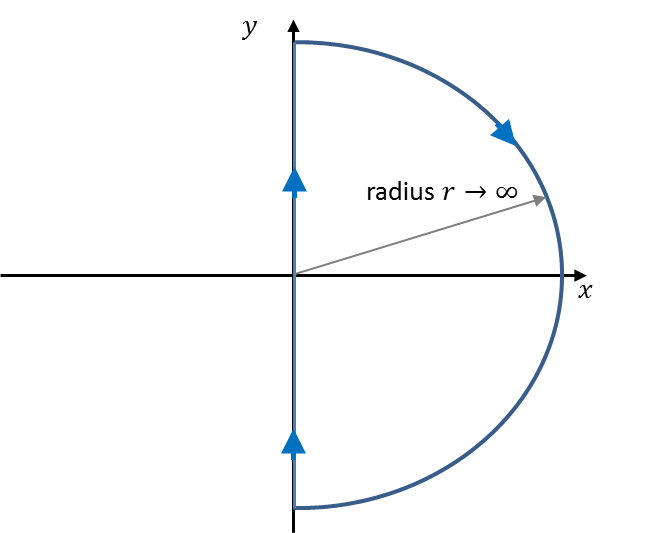
\includegraphics[width=0.7\linewidth]{nyquist_plot}
		\end{figure}
	\end{columns}
\end{frame}

\newcounter{sauvegardeenumi}
\newcommand{\asuivre}{\setcounter{sauvegardeenumi}{\theenumi}}
\newcommand{\suite}{\setcounter{enumi}{\thesauvegardeenumi}}

\begin{frame}
	\frametitle{Nyquist plot: physically realizable systems}
	\begin{enumerate}
		\item \textbf{Every physically realizable system is causal}\\
		This is logical: you cannot build a system that knows the future
		\item \textbf{Every causal system has a transfer function with a degree of the denominator that is larger than or equal to the degree of the numerator}\\
		Take for example the following transfer function:
		$$H(z)=\frac{b_2z^2+b_1z+b_0}{a_0z+a_1}$$
		The corresponding difference equation is: 
		$$a_0y_{n-1}+a_1y_n=b_0u_{n-1}+b_1u_n+b_2u_{n+2}$$
		It is non-causal, because the output depends on future input.
		\asuivre
	\end{enumerate}
\end{frame}

\begin{frame}
	\frametitle{Nyquist plot: physically realizable systems}
	\vspace{-8ex}
	\begin{enumerate}
		\suite
		\item \textbf{From the transfer function, we can easily show that the circle bow maps onto a point.}\\
		\begin{itemize}
			\item If the degree of the denominator is strictly higher than the degree of the numerator:\\
			If $s\rightarrow \infty$, then $P(s)C(s)\rightarrow 0$
			\item If the degree of the denominator is equal to the degree of the numerator:\\
			If $s\rightarrow \infty$, then $P(s)C(s)\rightarrow c$, a real number
		\end{itemize}
	\end{enumerate}
\end{frame}

\begin{frame}
	\frametitle{Nyquist plot: symmetry}
	\vspace{-12ex}
	The symmetry follows directly from the way $f(c)$ can be evaluated.\\
	\medskip
	Since the position of $f(c)$ only depends on the location of the poles and zeros, and those poles and zeros only occur symmetrically round the real axis, the Nyquist plot will be symmetrical round the real axis.
\end{frame}

\begin{frame}
	\frametitle{Nyquist plot}
	So we will only have to study the positive (or the negative) imaginary axis!\\
	\begin{itemize}
		\item The circular part maps onto one point, which is the same as where $j\omega$ maps onto
		\item The other half of the imaginary axis will give the mirror image of the studied half
	\end{itemize}	
	\begin{figure}
		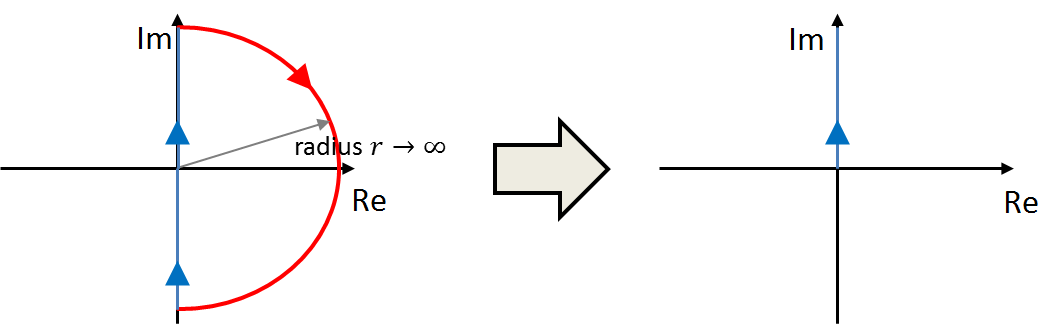
\includegraphics[width=1\linewidth]{plot}
	\end{figure}
\end{frame}

\begin{frame}
	\frametitle{Nyquist plot}
	\vspace{-6ex}
	Extracting the number of times $(-1,0)$ is encircled isn't that difficult anymore:
	\begin{itemize}
		\item You search for the image of $j0^+$
		\item You search for the image of $j\infty$
		\item You search for the positive real y for which $f(jy)$'s imaginary part changes sign
	\end{itemize}
	This information allows you to determine if you encircle $(-1,0)$\\
	Let's visualize this with a simple example, but of course you can use software to do this (e.g. nyquist in Matlab)
\end{frame}

\begin{frame}
	\frametitle{Nyquist plot: a simple example}
	Let's take the following open loop system: $$P(s)C(s)=\frac{1}{s^2-2s+2}$$
	Substitute s with $j\omega$  $$\frac{1}{-\omega^2-2j\omega+2}=\frac{1}{-\omega^2+2-2j\omega}\frac{-\omega^2+2+2j\omega}{-\omega^2+2+2j\omega}=\frac{-\omega^2+2+2j\omega}{(-\omega^2+2)^2+4\omega^2}$$
	\vspace{-2ex}
	\begin{itemize}
		\item $f(j0^+)=\frac{1}{2}$
		\item $f(j\infty)=0$
		\item Imaginary part: $\frac{2\omega}{(-\omega^2+2)^2+4\omega^2}=0\Rightarrow\omega=0$
	\end{itemize} 
	The real axis gets crossed 2 times: first at $\frac{1}{2} (\omega=0^+)$ and then at $0 (\omega=\infty) \rightarrow (-1,0)$ is not encircled
\end{frame}

\begin{frame}
	\frametitle{Nyquist plot: a simple example}
	Remember our open loop system: $$P(s)C(s)=\frac{1}{s^2-2s+2}.$$
	Z and P are respectively the number of zeros and poles of $1+P(s)C(s)$.\\
	The poles of $P(s)C(s)$ and $1+P(s)C(s)$ are the same ($P=2$ in our example).\\
	Since $(-1,0)$ is not encircled: $Z-P=0$, hence there are 2 zeros in the right half plane.\\
	Remember that the zeros of $1+P(s)C(s)$ are the poles of the closed loop system and thus, the unity feedback controller is unstable.
\end{frame}

\subsection{Poles on the imaginary axis}

\begin{frame}
	\frametitle{Nyquist plot: poles on the imaginary axis}
	Poles on the imaginary axis: why are they a problem?
	\begin{itemize}
		\item Take for instance the case with one pair of imaginary poles at $jc$ and $-jc$
		\item When coming close to $jc$, the argument will remain 0 and the gain will increase to infinity
		\item At $jc$ itself, the gain will be infinite, but the argument is undetermined, hence we cannot map this point
	\end{itemize}
	\begin{figure}
		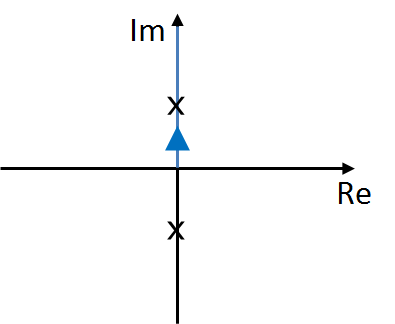
\includegraphics[width=0.35\linewidth]{imaginary_axis}
	\end{figure}
\end{frame}

\begin{frame}
	\frametitle{Nyquist plot: poles on the imaginary axis}
	How do we solve this?
	\begin{columns}
		\column{0.7\textwidth}
		\begin{itemize}
			\item Instead of going through the poles, we will evade them by an infinitesimally small amount (see figure)
			\item That way we do not have the problem of an undetermined mapping at the pole
			\item Since we avoid them by an infinitesimally small amount, we also know we will not wrongly avoid a pole that lies in the right half plane
		\end{itemize}
		\column{0.3\textwidth}
		\begin{figure}
			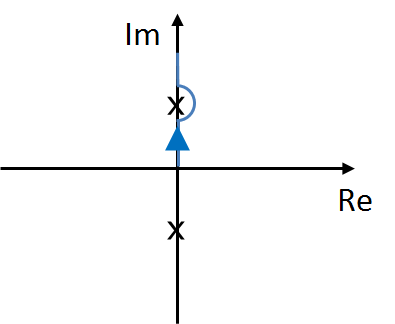
\includegraphics[width=1\linewidth]{avoid_pole}
		\end{figure}
	\end{columns}
	Now the Nyquist plot will go to infinity as the pole is approached, then the argument will change from 0 to $\pi$ as the semi-circle is traversed and then the Nyquist plot will return from infinity.
\end{frame}

\subsection{Discrete-time}

\begin{frame}
	\frametitle{Discrete-time case}
	The Cauchy argument principle still applies for discrete-time systems, since $P(z)C(z)$ also has the shape of a rational polynomial.\\
	The contour will have to encircle the entire complex plane except for the unity circle:
	\vspace{-4ex}
	\begin{figure}
		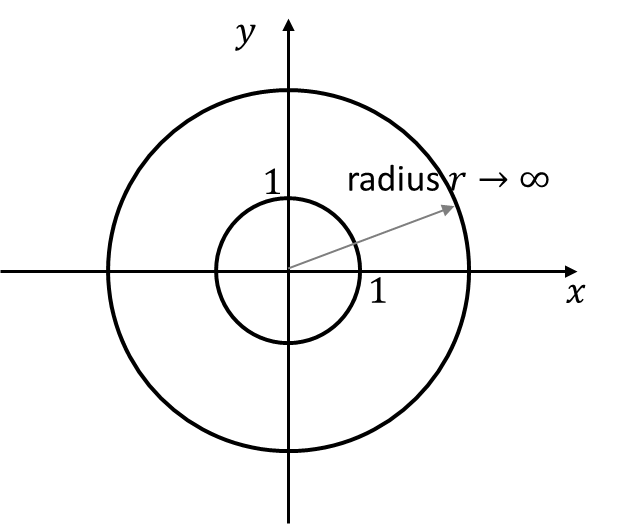
\includegraphics[width=0.55\linewidth]{discrete}
	\end{figure}
\end{frame}

\begin{frame}
	\frametitle{Discrete-time case}
	However, this is not a contour, but it can be solved with the following trick:\\
	the two horizontal pieces are both infinitely close to the real axis, that way they are identical but with opposite signs. They will cancel each other out.
	\vspace{-2ex}
	\begin{figure}
		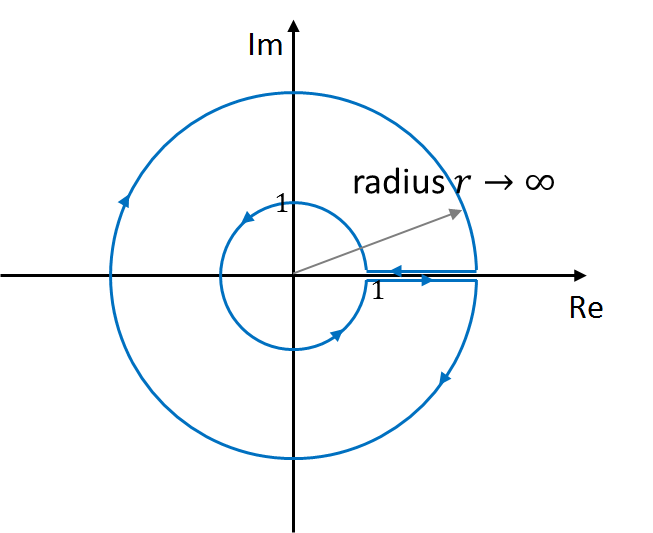
\includegraphics[width=0.5\linewidth]{discrete2}
	\end{figure}
\end{frame}

\section{Margins}

\begin{frame}
	\frametitle{Margins}
	\vspace{-6ex}
	The Nyquist plot allows us to determine the stability of the system\\
	We know the stability changes when $1+P(s)C(s)$ has an imaginary root (then the system is marginally stable).\\
	\medskip
	We can see such a root in the Nyquist plot of $P(s)C(s)$.\\ After all, the Nyquist plot is the image of the imaginary axis, so if there is a root on the imaginary axis, the Nyquist plot of $1+P(s)C(s)$ would go through 0 and the Nyquist plot of $P(s)C(s)$ would go through -1.
\end{frame}

\begin{frame}
	\frametitle{Margins}
	\vspace{-6ex}
	This explains why we can use the 'distance to -1' as a measure of stability.\\
	\medskip
	We will see two different stability margins, which can be easily read off the Nyquist diagram:
	\begin{itemize}
		\item \textbf{The gain margin}: the amount of extra gain you can allow before instability occurs (in dB)
		\item \textbf{The phase margin}: the amount of phase you can add before instability occurs
	\end{itemize}
\end{frame}

\begin{frame}
	\frametitle{Margins}
	\begin{figure}
		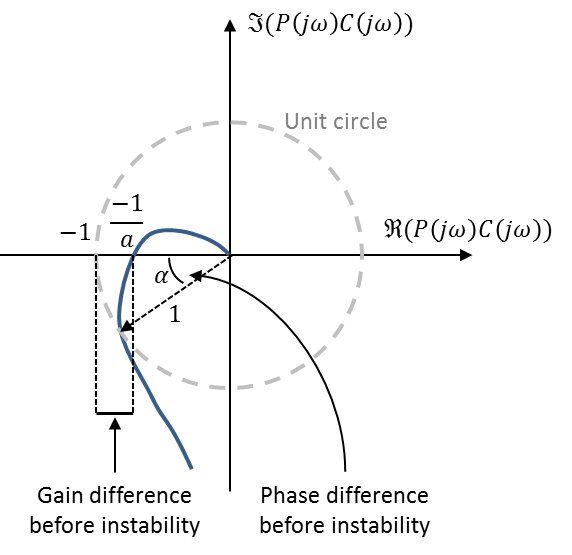
\includegraphics[width=0.6\linewidth]{margins}
	\end{figure}
\end{frame}

\subsection{Gain margin}

\begin{frame}
	\frametitle{Gain margin}
	\begin{columns}
		\column{0.5\textwidth}
		The gain margin is the amount of extra gain allowed before the system becomes unstable (or how much larger the gain has to be, before the system becomes unstable).\\
		\medskip
		The gain margin is \textbf{multiplicative}, so it is the factor you have to multiply the gain with, so the Nyquist plot goes through -1 in the w-plane.\\
		It will be expressed in dB $(20log_{10}K)$.
		\column{0.5\textwidth}
		\vspace{-4ex}
		\begin{figure}
			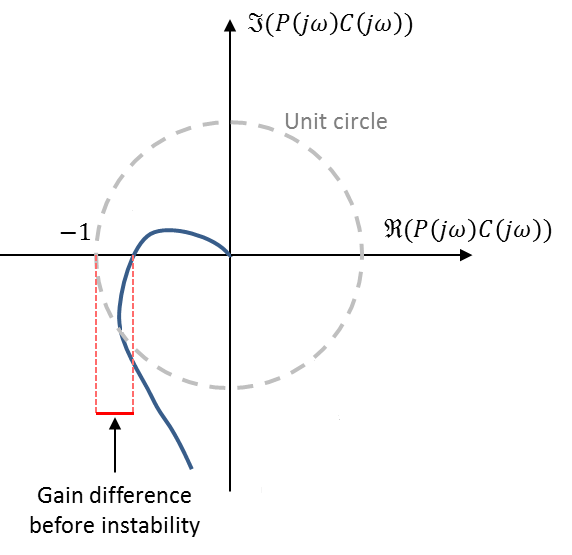
\includegraphics[width=1.1\linewidth]{gain_margin}
		\end{figure}
	\end{columns}
\end{frame}

\begin{frame}
	\frametitle{Gain margin}
	\vspace{-6ex}
	Let's look at it the following way:
	\begin{figure}
		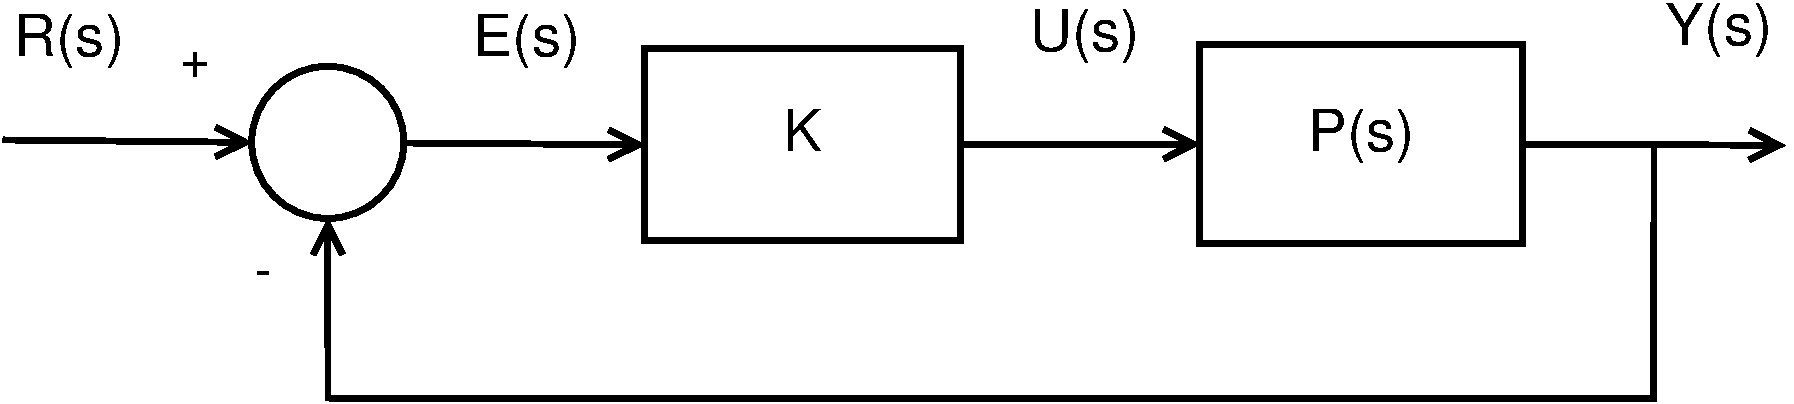
\includegraphics[width=0.8\linewidth]{closedloop2}
	\end{figure}
	The stability margin of $P(s)$ with unity feedback is the K for which the system above is marginally stable.
\end{frame}

\begin{frame}
	\frametitle{Gain margin}
	\vspace{-5ex}
	So $KP(s)$ should equal $-1$ for an imaginary $s=j\omega$.\\
	\bigskip
	This requires $\angle(KP(j\omega))=\angle P(j\omega)$ to equal $-180^{\circ}$. This $\omega_\pi$ is called the \textbf{Gain Crossover Frequency (GCF)}.\\
	K then has to be set such that $\big|KP(j\omega_\pi)\big|=1$.\\
	\bigskip
	So a large gain can lead to instability and this risk only exists when there exists a $\omega_\pi$ for which $\angle P(j\omega)=-180^{\circ}$.\\
	\medskip
	We will illustrate this with an example.
\end{frame}

\begin{frame}
	\frametitle{Gain margin: example}
	\vspace{-4ex}
	Consider the process $$P(s)=\frac{1}{s(s+2)}.$$\\
	We derive the argument as a function of $\omega$: $$\angle P(j\omega)=-tan^{-1}(\frac{\omega}{0})-tan^{-1}(\frac{\omega}{2})=-90^{\circ}-tan^{-1}(\frac{\omega}{2}).$$\\
	For this to equal to $-180^{\circ}$, it requires $\omega_\pi \rightarrow \infty$.\\ This makes $P(j\omega)=0$ and this means the gain margin is infinite.
\end{frame}

\begin{frame}
	\frametitle{Gain margin: example}
	This solution is shown in the Nyquist plot below:
	\vspace{-2ex}
	\begin{figure}
		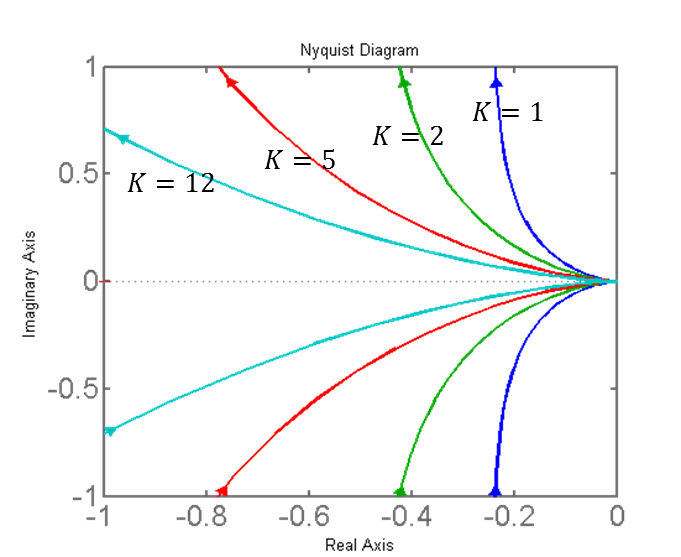
\includegraphics[width=0.6\linewidth]{gain_example}
	\end{figure}
	\vspace{-2ex}
	The only crossover with the real axis occurs at $\omega=0$ and that does not change with increasing K.
\end{frame}

\subsection{Phase margin}

\begin{frame}
	\frametitle{Phase margin}
	The phase margin is that amount of additional phase lag to bring the system to the verge of instability. 
	\vspace{-3ex}
	\begin{columns}
		\column{0.05\textwidth}
		
		\column{0.95\textwidth}
		\begin{figure}
			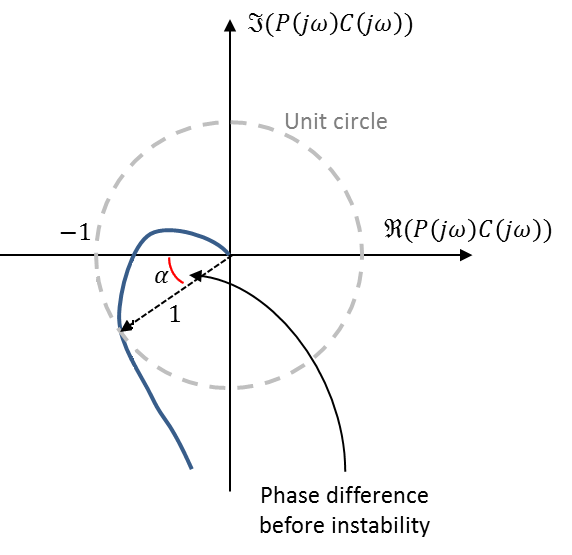
\includegraphics[width=0.6\linewidth]{phase_margin}
		\end{figure}
	\end{columns}
\end{frame}

\begin{frame}
	\frametitle{Phase margin}
	This can be interpreted as multiplying $P(s)$ with $e^{j\theta}$ until $-1$ is crossed, so $P(s)e^{j\theta}=-1$ for an imaginary $s=j\omega$.\\
	\medskip
	This requires $\big|P(j\omega)e^{j\theta}\big|=\big|P(j\omega)\big|$ to equal $1$. This $\omega_0$ is called the \textbf{Phase Crossover Frequency (PCF)}.\\
	$\theta$ then has to be set such that $$\angle(P(s)e^{j\theta})=\angle P(s) + \theta = -180^{\circ}.$$\\
	The gain margin is defined as positive, but that doesn't matter, because of the symmetry with respect to the real axis.\\
	If a rotation of $\theta$ degrees results in a crossing of $-1$, then a rotation of $-\theta$ does the same.
\end{frame}

\begin{frame}
	\frametitle{Phase margin: example}
	Consider the process \vspace{-2ex} $$P(s)=\frac{1}{s(s+2)}.$$
	We derive the modulus as a function of $\omega$: $$\big|P(j\omega)\big|=\frac{1}{\omega}\frac{1}{\sqrt{\omega^2+4}}.$$
	For this to equal to 1, we find $\sqrt{\omega^4+4\omega^2}=1$ or $\omega_0=\sqrt{\sqrt{5}-2}=0.486$.\\
	Now we need to find $\theta$ so $\angle(P(j\omega_0)e^{j\theta})=-180^{\circ}$.\\
	This results in $\theta = -180^{\circ}+tan^{-1}(\frac{\omega_0}{0})+tan^{-1}(\frac{\omega_0}{2})=-76.34^{\circ}$. \\
	This means the phase margin is $76.34^{\circ}$.
\end{frame}

\begin{frame}
	\frametitle{Phase margin: example}
	This solution is shown graphically in the Nyquist plot below:
	\begin{figure}
		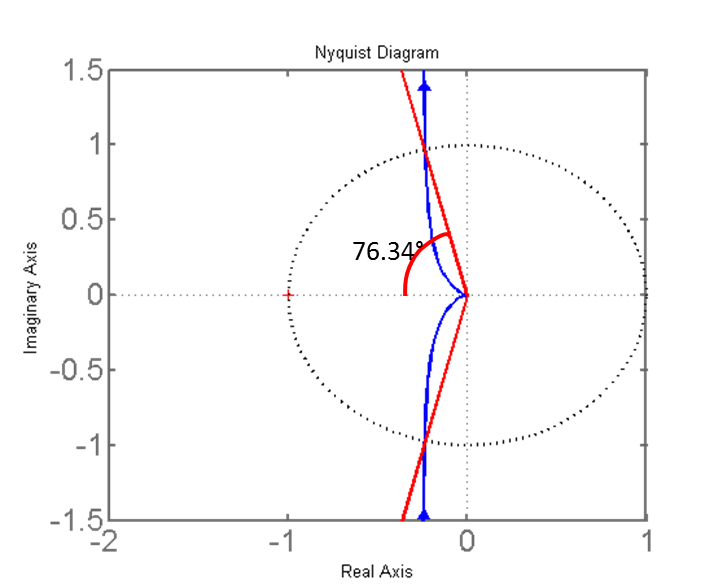
\includegraphics[width=0.65\linewidth]{phase_example}
	\end{figure}
\end{frame}

\begin{frame}
	\frametitle{What should the margins be?}
	\vspace{-4ex}
	Phase margin:
	\begin{itemize}
		\item This is more subtle than the gain margin
		\item If it is too small, instability might occur due to practicalities, the model is not perfect
		\item If it is too small, we get large overshoots and large oscillations that fade away very slowly
		\item Sometimes a good value is 60$^{\circ}$, but it is highly case-dependent
	\end{itemize}
	\bigskip
	A good margin does not offer certainty about the stability, whereas a bad phase margin (very large or very small) does give certainty about instability.
\end{frame}

\begin{frame}
	\frametitle{Margins using Bode plots}
	We can also easily derive the \textcolor{red}{gain margin} and \textcolor{blue}{phase margin} from the Bode plot of P(s)C(s):
	\vspace{-1ex}
	\begin{figure}
		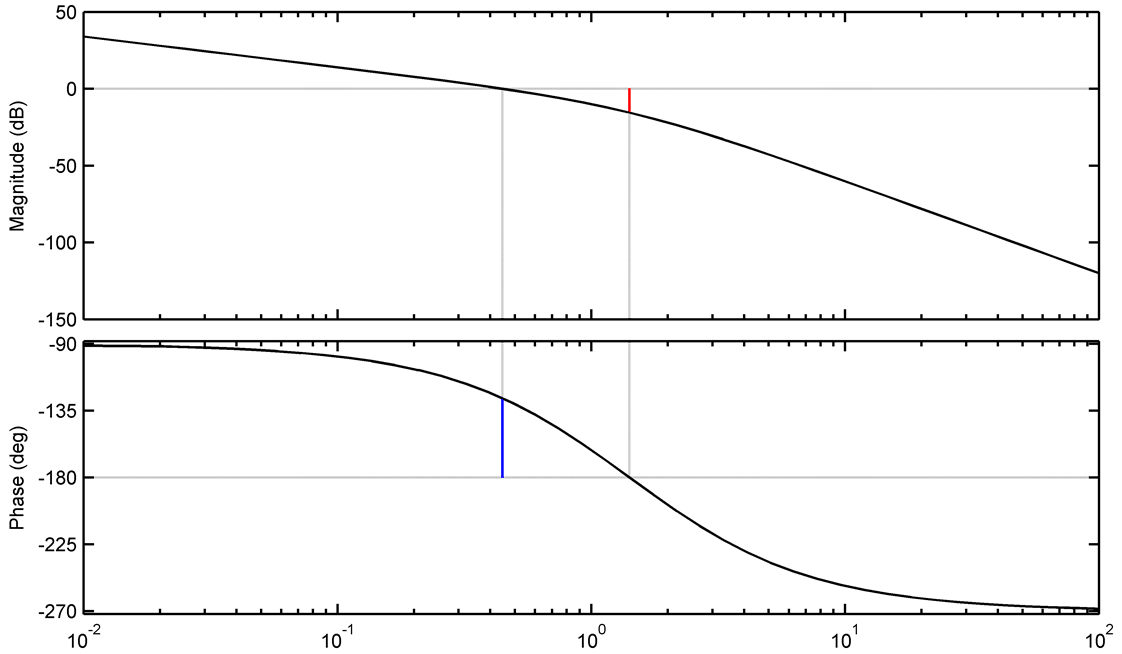
\includegraphics[width=0.87\linewidth]{bode}
	\end{figure}
\end{frame}

\subsection{Design example}

\begin{frame}
	\frametitle{Margins: design example}
	\begin{figure}
		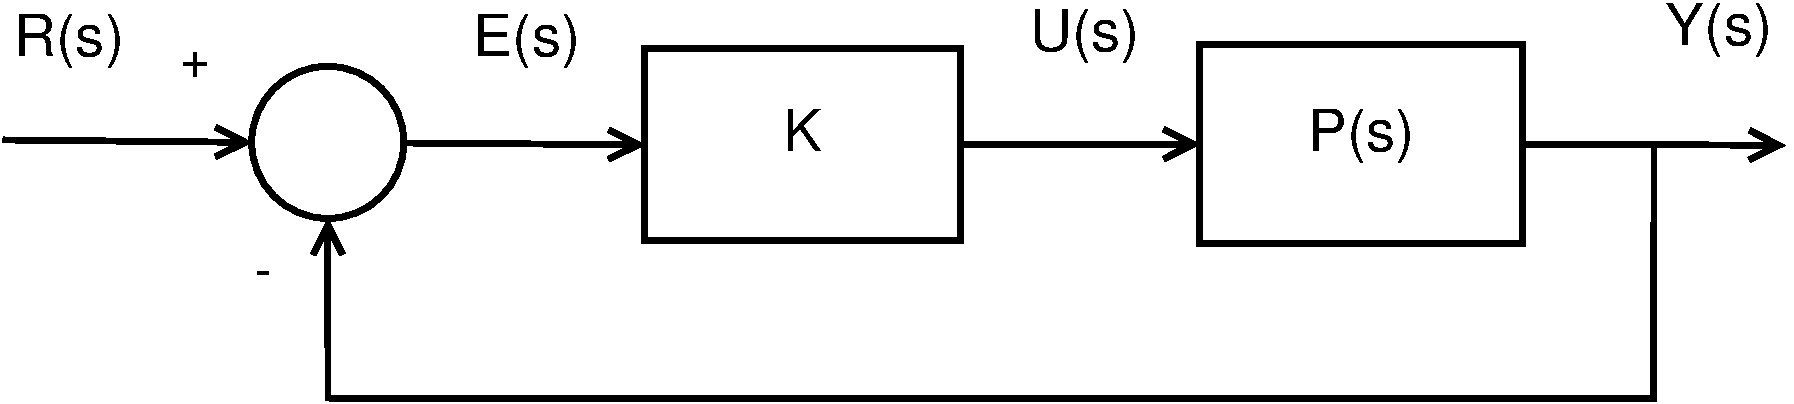
\includegraphics[width=0.8\linewidth]{closedloop2}
	\end{figure}
	Consider the following process $$P(s)=\frac{1-s}{(1+s)^2}.$$
	Design a simple proportional controller K with a phase margin of 45$^{\circ}$.
\end{frame}

\begin{frame}
	\frametitle{Margins: design example}
	We find $\omega$ by demanding
	\begin{align*}
		\angle(P(j\omega)e^{\frac{j\pi}{4}})&=-180^{\circ}\\
		45^{\circ}+tan^{-1}(-\omega) -tan^{-1}(\omega)-tan^{-1}(\omega) &=-180^{\circ}\\
		-3tan^{-1}(\omega)&=-225^{\circ}\\
		\omega &= tan(75^{\circ})=3.73
	\end{align*}
	Now we can find K (which doesn't influence the argument) by setting $\big|KP(j\omega)\big|=1$:
	$$K\frac{\sqrt{\omega^2+1}}{\sqrt{\omega^2+1}^2}=\frac{K}{\sqrt{\omega^2+1}}=\frac{K}{3.86}=1\rightarrow K=3.86=5.87 dB$$
\end{frame}

\begin{frame}
	\frametitle{Margins: design example}
	We can also do this graphically with the Nyuist plot.\\
	\medskip
	First determine the point that corresponds to $\theta = 45^{\circ}$.\\
	Then determine the modulus, K is the inverse of that modulus.
	\vspace{-2ex}
	\begin{figure}
		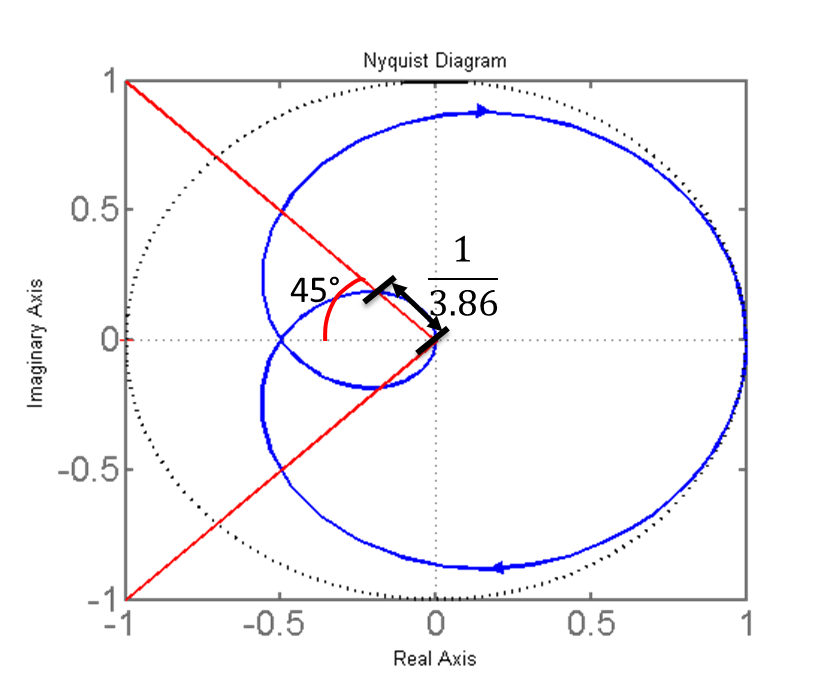
\includegraphics[width=0.6\linewidth]{design_example}
	\end{figure}
\end{frame}

\begin{frame}
	\frametitle{Summary}
	\vspace{-10ex}
	\begin{itemize}
		\item The Nyquist stability criterion came to existence as a cheap alternative to determine stability of a closed loop system with unity feedback
		\item It also shows the phase margin and the gain margin, which are used to measure the stability of the system
		\item It is relevant as a design tool, as shown in the last example
	\end{itemize}
\end{frame}
